\doublespacing
\chapter{MARCO TEÓRICO}
\spacing{1.5}
\lettrine[lines=4, slope=0.2em, findent=0.2em, nindent=0.6em]{E}l presente capitulo tiene como propósito presentar al lector algunas investigaciones y conceptos relacionados con IA, específicamente ML y en salud particularmente de ACV Isquémico, conceptos claves para esta investigación. \\
\par La organización del capítulo se encuentra de la siguiente manera, inicialmente, veremos ML y sus técnicas clásicas, pues consideramos estas podrían ser la respuesta a nuestra problemática junto a Deep Learning (DL), posteriormente nos enfocaremos en algunos términos de salud que nos ayudaran a resolver y entender de mejor forma la raíz del problema. 
\\

\doublespacing
\section{Inteligencia Artificial}
\spacing{1.5}
Las matemáticas nos han ayudado a interpretar y entender nuestro medio ambiente y poder ser capaz de predecir algunos sucesos en áreas como la cosmología o naturaleza o problemas incomprendidos por los humanos \cite{Grazia2022}. Hoy en día contamos con el área de las ciencias de la computación que fue creada hace solo un par de décadas atrás, siendo una de las ciencias más nuevas y que tiene gran valoración en la actualidad. En las ciencias de la computación podemos encontrar varias áreas aplicadas, de las cuales la IA es una de las más cotizadas, porque involucra en su relación la matemática con filosofía, biología, lingüística, entre otras, pudiendo resolver los problemas con distintos tipos de algoritmos \cite{Grazia2022}.\\
\par La IA llegó para resolver tareas que el ser humano realiza como tareas cotidianas básicas y complejas. Los algoritmos de IA, se basan en el aprendizaje automático, siendo que cada vez las máquinas pueden aprender por ellas mismas algunas cosas, es así que los humanos dejaremos de perder nuestro tiempo programando reglas para lidiar con muchas combinaciones de datos y situaciones que aparecen en nuestro mundo. Pues es así, que aprender los algoritmos, es fijarse como aprender desde pequeños, como el aprendizaje por refuerzos, que involucra una serie de técnicas de aprendizaje automático que las máquinas usan en sistemas artificiales \cite{Carola}.\\
\par En la IA, para que los modelos funcionen existen modelos neuronales y estos son los que determinan cómo se conectan los datos predictores con los objetivos a través de capas ocultas, y estas a su vez contienen unidades no observables \cite{IBM}. Dentro de la IA, convive un sub conjunto llamada ML y su vez, dentro de ML vive un subconjunto llamado DL. Estos sub conjuntos interactúan con lo que es el Data Science y el Big Data, haciendo de las aplicaciones una variada gama de aplicaciones \cite{moreno2021diseno}.\\

\begin{figure}[h]
	\centering
	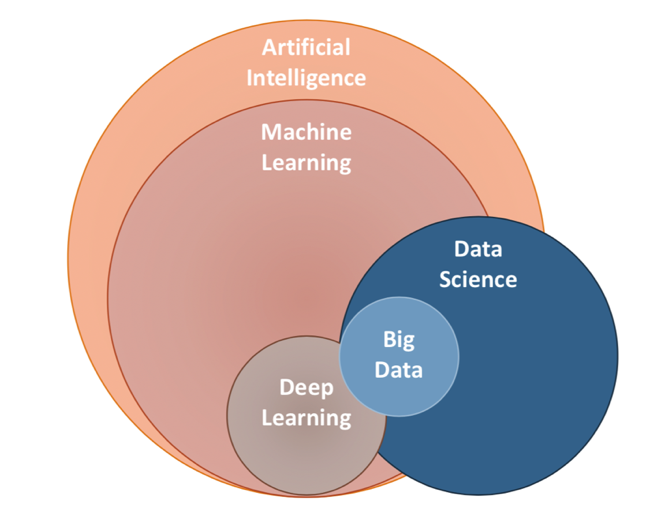
\includegraphics[scale=0.51]{img/Marco Teorico/Expertiz.png} 
	\caption{Diagrama de Venn con los subcojuntos de la IA}
\end{figure}


\doublespacing
\section{Machine Learning}
\spacing{1.5}
Los problemas por computadora siempre son solucionado con un algoritmo que le indica a la maquina los pasos a seguir para dar solución a dicho problema, en un ejemplo clásico podemos usar un algoritmo de búsqueda, donde el dato a buscar seria la entrada y su salida seria la respuesta a que si se encontró o no y en cuanto tiempo, es bien conocido que para resolver el problema de búsqueda existen variados algoritmos, algunos más eficientes que otros, aplicables a un contexto u otro de mejor forma, solucionando el mismo problema.\\
\par Asimismo, existen tareas cotidianas como lo son la publicidad en el celular, como muestra cosas que me gustan o que he estado pensando en comprar, esto es gracias a algoritmos de ML que captan la información de navegación de nuestro celular y nos muestra lo que nosotros estamos deseando o es de nuestro interés.\\
\par En el año 1959, Arthur Samuel, definió el concepto de ML como:

\begin{quote}
	\emph{"Un campo de estudio que le entrega a los computadores la habilidad de aprender sin haber sido explícitamente programado para eso"}
\end{quote}


Tom M. Mitchell define el ML en uno de sus libros como:
\begin{quote}
	\emph{“El estudio de algoritmos de computación que mejoran automáticamente su rendimiento gracias a la experiencia. Se dice que un programa informático aprende sobre un conjunto de tareas, gracias a la experiencia y usando una medida de rendimiento, si su desempeño en estas tareas mejora con la experiencia”}
\end{quote}

\par Es decir, estos algoritmos aprenden y mejoran solos gracias a la experiencias pasadas a diferencia de modelos que un experto puede asignar reglas y modela gracias a sus conocimientos.\\
\par El ML es el subconjunto de la IA, utilizándose para que las máquinas aprendan de grandes volúmenes de datos. Una vez adquirido el conocimiento, este puede ser empleado a otro conjunto de datos, recibiendo una atención cada vez mayor de un modelo que es capaz de interpretar los datos con mejor capacidad cada vez \cite{murdoch2019interpretable}.\\

\doublespacing
\subsection{Machine Learning: Tipos de Aprendizajes}
\spacing{1.5}
Para ML existen algunos enfoques para trabajar, los cuales son los más usados el aprendizaje supervisado y el aprendizaje no supervisado.\\


\doublespacing
\subsubsection{Aprendizaje Supervisado}
\spacing{1.5}
Este enfoque es un método de análisis de datos que necesita de algoritmos que aprendan a través de entrenamiento, en el cual el programa es alimentado con datos etiquetados tanto con los atributos como la variable objetivo de cada iteración.\\
\par En el aprendizaje supervisado del algoritmo existen dos tareas comunes que son la clasificación y regresión. En las tareas de clasificación las variables objetivo, son valores etiquetados de manera nominal, mientras que en las tareas de regresión la variable objetivo tiene un dominio dentro de los números reales y por lo tanto pueden tomar infinitos valores \cite{murdoch2019interpretable}. \\


\doublespacing
\subsubsection{Aprendizaje No Supervisado}
\spacing{1.5}
El aprendizaje no supervisado tiene datos sin etiquetar que el algoritmo tiene que entender por si mismo, el propósito es descubrir patrones ocultos en ellos. Si nosotros le pedimos a nuestro programa \textit{"predecir Y para nuestros datos A"} nosotros deberíamos \textit{“pedirle que nos provea de la información de nuestros datos A"} \cite{murdoch2019interpretable}.\\
\par Las tareas más comunes dentro del aprendizaje no supervisado son el \emph{clustering} y \emph{dimensión reduction}, los cuales no son objeto de nuestro estudio por lo que sólo son mencionados en esta parte del documento.\\


\doublespacing
\subsection{Técnicas de Clasificación}
\spacing{1.5}
Para que nuestro modelo de ML funcione, debemos categorizar los datos de entrada y salida, reconociendo atributos del elemento a clasificar y utilizando el conocimiento adquirido durante el entrenamiento del algoritmo para asignar un valor a la variable objetivo de dicho elemento.\\
\par La clasificación de datos es un proceso que posee dos etapas:\\
\par La \textit{primera} es la etapa de aprendizaje, la cual los datos ingresan al modelo son entrenados con una serie de datos que sirven de base del algoritmo, logrando que se entrene con un set de entrenamiento que no son mas que tuplas de datos etiquetados tanto en sus atributos como en su variable objetivo.\\
\par La \textit{segunda} etapa, el algoritmo ya ha sido entrenado con los datos de entrenamiento y esta listo para su clasificación de una variable cualquera, siendo capaz de tomar algunos atributos de la variable, analizarlos y tomar una decisión basándose en los datos que fueron entregados anteriormente.\\
\par En la clasificación veremos algunas de las técnicas clásicas de ML, pertenecientes al enfoque de los algoritmos de aprendizaje supervisado, definiendo brevemente cada una de ellas \cite{murdoch2019interpretable}.\\


\doublespacing
\subsection{Decision Tree (Árbol de Decisión)}
\spacing{1.5}
Este algoritmo que se utiliza como herramienta de apoyo gráfico o modelo de decisiones con sus posibles consecuencias, también a veces son representados los costos y su posible utilidad (CART, Classification and Regression Trees). Este método se crea particionando la entrada recursivamente en distintas ramas, siendo que la idea es crear un camino desde la raíz hasta las hojas, donde cada nodo podría ser una condición, así si se cumple la condición se sigue por el camino de decisión o por la otra rama si no se llegará a cumplir la condición \cite{Teknomo2015}.\\
\par La creación del modelo se puede representar con la siguiente ecuación:\\

\begin{Large}
	\begin{equation}
		f(x)=E[y|x]=\sum_{m=1}^{M}w_{m}I(x \in R_{m})=\sum_{m=1}^{M}w_{m}\phi(x;v_{m})
	\end{equation}
\end{Large}
\par $R_{m}$ representa la región de $m$.
\par $w_{m}$ es respuesta media a esa región.
\par $v_{m}$ codifica la elección de la variable por la que dividir y el valor límite de la división.\\
\par  La forma gráfica del modelo se puede representar de la siguiente forma en condiciones:\\

\begin{figure}[h]
	\centering
	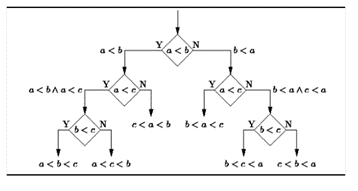
\includegraphics[scale=1]{img/Marco Teorico/arbol de desicion.png} 
	\caption{Forma Gráfica de un Árbol de Desiciones}
\end{figure}
\par Las condiciones se dan como alternativas de caminos a seguir.\\

\doublespacing
\subsubsection{Usos para los Decision Tree}
\spacing{1.5}
Al ser de fácil implementación, los Decision Tree son usados en diversas áreas, siendo las instituciones financieras las más comunes, ayudando a clasificar clientes, estableciendo sus riesgos o posibilidades financieras.\\
\par En el área de la salud son empleados para diagnósticos de infecciones a la sangre o predicción de ataque al corazón en pacientes de alto riesgo.\\
\par En el área de entretenimiento son ampliamente usados como métodos de seguimiento de movimiento y a su vez como método de reconocimiento facial.

\doublespacing
\subsubsection{Ventajas y Desventajas}
\spacing{1.5}
Principalmente las ventajas de esta técnica de ML es su bajo costo computacional y simple interpretación de resultados. \\
\par La mayor desventaja es que la técnica es propensa a caer en el sobreajuste, siendo a veces manipulada por quien lo implemente \cite{Harrington2012}.\\


\doublespacing
\subsection{Naïve Bayes (Redes de Bayes)}
\spacing{1.5}
La clasificación de Naïve Bayes es un algoritmo probabilístico basados en la probabilidad condicional y teorema de Bayes con atributos fuertes y de independencia entre características \cite{Shafe}. Este modelo es de fácil construcción y funciona bien en comparación a los métodos más sofisticados de clasificación, lo que lo hace particularmente útil en los diferentes campos investigativos \cite{Vembandasamy2015}.\\
\par La fórmula condicional se expresa:\\
\begin{Large}
	\begin{equation}
		P(A|B)=\frac{P(A \cap B)}{P(B)}= \frac{(\frac{\#casos favorables A \cap B}{\#casos posibles})}{(\frac{\#casos favorables B}{\#casos posibles})}
	\end{equation}
\end{Large}\\
\par Desarrollando la ecuación nos queda:\\
\begin{Large}
	\begin{equation}
		P(A|B)=\frac{P(B|A)*P(A)}{P(B)}
	\end{equation}
\end{Large}\\
\par Donde cada evento es tomado como:\\
\begin{large}
	\begin{equation}
		P(A|B)= P(B_{1}|A) \times P(B_{2}|A) \times … \times P(B_{n}|A) \times P(A)
	\end{equation}
\end{large}\\
\par $P(A|B)$ es la probabilidad posterior de la clase (objetivo) dado el predictor (atributo).
\par $P(A)$ es la probabilidad previa de clase.
\par $P(B|A)$ es la probabilidad, que es la probabilidad de la clase dada del predictor.
\par  $P(x)$ es la probabilidad previa del predictor.\\

\par Las Redes de Bayes se generan de reglas de decisión donde participan activamente las probabilidades que ocurren referente a eventos, siendo que en base a esas probabilidades y resultados obtenidos, se toman decisiones sobre cual arco de red moverse, al final del proceso, el resultado será dado por el valor del nodo final de la red.\\


\doublespacing
\subsubsection{Ventajas y Desventajas}
\spacing{1.5}
La gran sencilles para enfrentar problemas lo hace ser una de las técnicas clásicas de ML más fácil de interpretar al momento de los resultados, además debemos agregar al valor que son fáciles de construir y toma evidencia de muchos atributos para realizar la predicción final.\\


\doublespacing
\subsection{Logistic Regression (Regresión Logística)}
\spacing{1.5}
El algoritmo Logistic Regression modela la relación entre distintas variables utilizando una medida de error que se intentará minimizar en un proceso iterativo para poder realizar predicciones acertadas, llevando a cabo una clasificación binaria con una distribución Bernoulli en vez de Gaussian y después realiza una combinación lineal de las variables en un rango de 0 a 1 \cite{ Stoltzfus2011}.\\
\par La ecuación lineal se debe ajustar:\\
\begin{Large}
	\begin{equation}
		y(X)=W^{T}X + \epsilon = \sum_{j=1}^{D}w_{j}x_{j} + \epsilon
	\end{equation}
\end{Large}\\ 
\par $W^{T}X$ representa el producto escalar de entrada X.
\par $W$ e $Y$ son vectores de pesos $\in$ $\lbrace 0,1 \rbrace$.\\

\par Ahora mostrando la distribución de Bernoulli:\\
\begin{Large}
	\begin{equation}
		p(y|x,w) = Ber(y|u(x))
	\end{equation}
\end{Large}
\begin{center}
	El resultado del intervalo quedaría $0 \leq u(x) \leq 1$.\\
\end{center}
\par El resultado de la ecuación nos ayudará a predecir valores con la mejor respuesta a partir del menor error posible, teniendo un valor continuo entre 0 y 1. Si existe un valor mayor o igual a 0.5, la clase será 1, en cambio si es menor será 0. Todo esto ocurre porque el algoritmo de Logistic Regression predice un valor en vez de una clase en función de las variables utilizadas.\\

\doublespacing
\subsubsection{Ventajas y Desventajas}
\spacing{1.5}
La Regresión Logística al igual que las técnicas anteriores es fácil de implementar, interpretar y muy eficiente al momento de entrenar, incluyendo que no hace suposiciones sobre distribuciones de clases en el espacio de características y es muy rápido para clasificar registros desconocidos.\\
\par Las principales desventajas de esta técnica radican en si el número de observaciones es menor que el número de características, no se debe utilizar la regresión logística; de lo contrario, puede provocar un sobreajuste y la difícil obtención de relaciones complejas.  Además de los algoritmos más potentes y compactos, como lo son las redes neuronales, las cuales pueden superar fácilmente este algoritmo. \\


\doublespacing
\subsection{Support Vector Machine (Máquina de Vectores de Soportes)}
\spacing{1.5}
Si bien es cierto que los algoritmos para dar un resultado de aprendizaje automático deben ser capaces de aprender de su pasado y así poder predecir su futuro, de manera que las Support Vector Machine (SVM), están para ayudarnos a la regresión a base de un conjunto de muestras, donde existen dos valores generales, uno lo compone una matriz con variables explicativas de la muestra y el otro valor general está con el valor que se espera de la muestra. En este método, una función elige la predicción del valor esperado del caso mediante una entrada de datos  \cite{Dantas2021}.\\

\doublespacing
\subsection{Artificial Neural Networks (Redes Neuronales Artificiales)}
\spacing{1.5}
Aunque no será parte de las técnicas para análizar los datos, se considera importante para este trabajo poder mencionarla. La Artificial Neural Networks (ANN), se caracteriza por su aprendizaje supervisado y no supervisado, eso quiere decir que es un modelo que trabaja con ML en su forma base, aunque de igual forma se ocupa para DL, posee una arquitectura de procesadores múltiples interconectados \cite{salas2004redes}. Mediante la técnica señalada para el aprendizaje de una ANN, podemos guiarnos de dos formas de organizar las capas ocultas, la cuales son los perceptores multicapa (PMC) \cite{Borracci2021}, encargado de las relaciones más complejas vía mayor coste de tiempo de entrenamiento, y la función de base radial (RBF) con una potencia de predicción reducida. De este modo, los métodos de aprendizaje que se emplean por lo regular son arquitecturas de redes neuronales tradicionales, donde solo se contienen dos o tres capas ocultas, imitando la operación que realiza el cerebro (Azath et al., 2020), en cambio, el DL aprenden sobre la marcha y su arquitectura puede llegar a tener 150 capas ocultas. \\

\doublespacing
\subsection{Deep Belief Network (Red de creencias profundas)}
\spacing{1.5}
Aunque no será parte de las técnicas para análizar los datos, importante conocer esta técnica. Esta red conlleva a un método de ML que nos ayuda con el rol probabilístico, que se ejecuta en los múltiples niveles de capas y variables ocultas, conectándose entre las capas visibles y ocultas, pero no en las capas visibles – visible u oculta – oculta \cite{PuertaBarrera2015}.\\

\doublespacing
\subsection{Feedforward Artificial Neural Network (Red Neuronal de Retroalimentación)}
\spacing{1.5}
Aunque no será parte de las técnicas para análizar los datos, importante conocer esta técnica. Las Feedforward Artificial Neural Network (FANN) es la sucesora de ANN, trabajándose en diversos campos y aplicándose más a lo que es el DL. La diferencia de la FANN en contraste con su predecesora es su arquitectura con un conjunto de neuronas organizadas por capas y su algoritmo de entrenamiento que se ajusta a la muestra, ejecutando el proceso de aprendizaje que la hace crecer más \cite{salas2004redes}.\\

\doublespacing
\subsection{Recurrent Neural Networks (Redes Neuronales Recurrentes)}
\spacing{1.5}
Aunque no será parte de las técnicas para analizar los datos, es importante que conozcamos esta técnica. Las Recurrent Neural Networks (RNN), son reconocidas por obtener información de datos secuenciales como lo son el procesamiento del lenguaje natural, videos y subtitulación de imágenes. Las RNN su modelo asigna parámetros únicos para representar a cada dato en una secuencia \cite{arana2021redes}, para poder tener el control y no sufrir interrupciones sobre la secuencia. Su arquitectura es multicapa que comparte pasos entre los datos espaciados secuencialmente, para poder unir la información.\\
\par Su arquitectura se va incrementando con la conexión de nodos adyacentes a través de la adición de ciclos dentro de la red.\\


\doublespacing
\section{Deep Learning (Aprendizaje Profundo)}
\spacing{1.5}
Las técnicas de ML, están limitadas en el procesamiento de los datos naturales en forma cruda y para dar solución a la problemática se creó el aprendizaje profundo. La comprensión de la IA y como puede llegar a igual a los comportamientos humanos, inclusive en el aprendizaje, a veces superándonos, fue un gran acontecimiento que se debe a la gran contribución de Alan Turing \cite{Carola}. El DL como subconjunto del ML entra en acción cuando los datos tienen demasiadas características, son enormes, se requiere de un nivel de precisión altísima y el ML no puede ofrecer completamente los resultados deseados.\\

\doublespacing
\subsection{Entrenamiento de Redes Neuronales del Deep Learning}
\spacing{1.5}
La forma para poder crear y entrenar los modelos de DL depende del método a implementar, para ello, al mismo tiempo, existen concepciones de procesos similares que son para los modelos basados en este tipo de aprendizaje.\\
\par En primera instancia, se inicia con el entrenamiento desde cero, tomando un conjunto amplio de datos etiquetados, diseñando la red arquitectónica que aprenda \cite{Pang2017}, de igual modo se determina la transferencia de aprendizaje, donde implica el ajuste detallado de un modelo previamente que ya fue entrenado, como puede ser GoogleLeNet que es un sistema que está relacionado con el DL. \\
\par En segunda instancia, para trabajar con cantidades masivas de datos se requiere una extracción de características que será un enfoque más especializado, en vista de que las capas con sus tareas asignadas gozan de ciertas características de aprendizaje, estas características se pueden extraer en cualquier momento para darle mayor flexibilidad, clasificación y posible capacidad de regresión, como lo es el ejemplo de las máquinas de vectores de soporte (SVM) \cite{Dong2018}.\\
Por último, lo relacionado respecto al tiempo es fundamental, dado que los principales problemas que enfrenta la tecnología es el tiempo, siendo que hay algoritmos que quizás se pueden demorar hasta semanas con los datos. Para esto, el uso de recursos de cómputo mediante GPU, reduce el tiempo para entrenar una red y acota el tiempo de entrenamiento para resolver un problema, perfeccionando el modelo de DL \cite{Pang2017}.\\

\doublespacing
\subsection{Convolutional Neural Networks (Redes Neuronales Convolucionales)}
\spacing{1.5}
El DL ha demostrado muy buenos resultados para la resolución de problemas, en cambio, las limitaciones, sobre todo en el campo de la imagenología, ha hecho que se elabore un método diferente para que exista un análisis más preciso al momento de analizar la imagen. Este método se llama Convolutional Neural Networks (CNN), que tiene una arquitectura con mejor rendimiento para las tareas complejas relacionales \cite{Pena-Torres}. \\
\par Desde el año 2012, las arquitecturas basadas en CNN para visión artificial han crecido muchísimo; sin embargo, no todas han sido eficientes para ocuparse en tareas de visión artificial (Figueroa Flores, 2021), siendo el Grupo de Geometría Visual (VGG) de la Universidad de Oxford \cite{Simonyan2015} una de las arquitecturas más utilizadas para las tareas de procesamiento de visión artificial. \\
\par Las CNN se forman usando tres tipos de capas, los cuales son las capas convolucionales, capas de pooling y capas totalmente conectadas.\\

\begin{figure}[h]
\centering
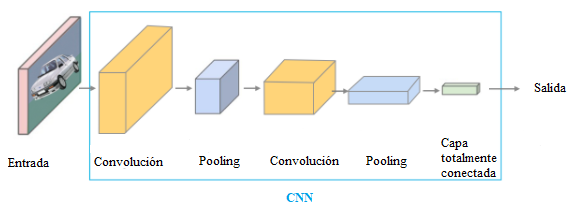
\includegraphics[scale=0.7]{img/Marco Teorico/convulcioinales.png}  
\caption{Descripción del funcionamiento de una red neuronal convolucional (CNN) }
\end{figure}

\par Para la CNN existen dos arquitecturas básicas de CNN, la cuales son CNN que entrega una salida para toda la imagen, como en la figura anterior y la Fully Convolutional networks que posee un codificador y decodificador, entrega una compresión de la información y su salida es por pixel. En las arquitecturas CNN exiten varios ejemplos, como lo son AlexNet, entrenado con ImageNet, GoogLeNet donde posee 22 capas y sus neuronas son más complejas, entre otras \cite{NIPS2012_c399862d}.\\

\begin{figure}[h]
\centering
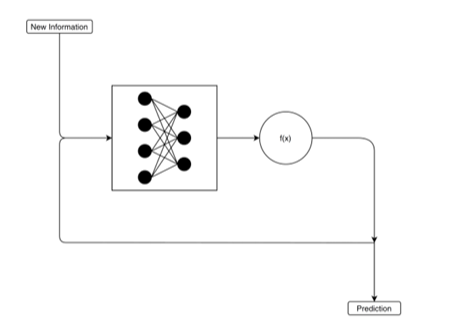
\includegraphics[scale=0.8]{img/Marco Teorico/rnn.PNG}  
\caption{Diagrama de grafo ciclico de una red neuronal recurrente (RNN) }
\end{figure}

\doublespacing
\subsection{Neural Networks for Scarce Data Domains  (Redes neuronales para dominios de datos escasos)}
\spacing{1.5}
En algunos casos, los modelos no contemplan con demasiados datos y por ende no se puede ser preciso con total certeza de la predicción de los resultados de la tarea. Por tanto, esto que se apunta a crear modelos que existan pocas muestras etiquetadas disponibles \cite{Carola}. Fei-Fei et al. \cite{Fei-Fei2006} demostraron que es posible aprender nuevas categorías, una o pocas muestras por clase, aprovechando las categorías aprendidas anteriormente. \\

\doublespacing
\section{Dataset}
\spacing{1.5}
\par Los Dataset están relacionados con el Big Data y con el procesamiento de datos, porque son datos tabulados, donde cada columna representa una variable y las filas datos, en consecuencia, el Dataset es una base de datos que se puede obtener de plataformas \cite{Astudillo2021}. Los Datasets, nos ayudan a trabajar con volúmenes de datos más pequeños, ya que la principal función de los Datasets es que hacen referencia a una única base de datos de origen. Estos Datasets se clasifican según su origen y formato, que son utilizados según las necesidades de su modelo, existiendo tipos de archivo, carpeta, bases de datos y web, cada uno con su formato. Se pueden encontrar con grandes voleumnes de información con fuentes privadas como gratuitas, siendo una de ellas Google Dataset Seach.\\


\doublespacing
\section{Aspectos de la salud y la enfermedad}
\spacing{1.5}
La salud es una de los aspectos más importantes en la vida, muchas veces nuestra salud se ve afectada por factores externos o internos a nuestra persona. “Este concepto involucra un estado completo de bienestar físico, mental y social, y no solamente la ausencia de afecciones o enfermedades” (Wold Health Organization, 1946). Estas palabras son relatadas en la conferencia del 46’ que hacen la referencia a que la persona no solo se compone de un estado físico, sino que hay más aspectos para sentirse saludable, ya que, si uno llegará a fallar, habría un déficit en la persona y poco a poco empezaría a carecer de un estado equilibrado que lo proporciona la salud. \\

\doublespacing
\subsection{Accidente Cerebro Vascular}
\spacing{1.5}
\par Un Accidente Cerebro Vascular es la detención del flujo de sangre a una parte del cerebro. En ocasiones se le llama como “Ataque Cerebral”, al igual, si el flujo sanguíneo se detiene por más de pocos segundos, el cerebro no recibirá nutrientes ni oxígeno, causando una muerte y un daño permanente en la zona afectada \cite{Garcia2019}.
\par Existen dos tipos de ACV, los cuales son Isquémicos y Hemorrágicos.\\

\doublespacing
\subsection{Accidente Cerebro Vascular Isquémico}
\spacing{1.5}
\par Los isquémicos es el más común, generalmente, es causado por un coagulo sanguíneo (masas que se presentan cuando la sangre se endurece, pasando de liquida a sólida) que bloquea el vaso sanguíneo del cerebro, empezando a morir en cuestión de minutos las células cerebrales. Existen los ACV Isquémicos transitorios y los permanentes \cite{Garcia2019}, diferenciándose en que los transitorios solo es cuando la sangre no llega al cerebro por unos instantes y el permanente es cuando ya tiene un tiempo prolongado el ACV, también conocido como Infarto Cerebral.\\

\doublespacing
\subsection{Síntomas ACV Isquémico}
\spacing{1.5}
\par Los síntomas de un ACV Isquémico pueden ser:
	\begin{itemize}
		\item Entumecimiento o debilidad repentina de la cara, brazo o pierna (especialmente en un lado del cuerpo).
		\item Confusión repentina, dificultad para hablar o entender el lenguaje.
		\item Dificultad repentina para ver con uno o ambos ojos.
		\item Problemas para caminar repentino, mareos, pérdida de equilibrio o coordinación.
		\item Problemas para caminar repentino, mareos, pérdida de equilibrio o coordinación.\\
	\end{itemize}
	
\doublespacing
\subsection{Categorías de los ACV}
\spacing{1.5}
\par En los ACV para ayudar a optimizar el tratamiento específico, existen categorías que son identificadas por la escala de TOAST \cite{Adams1993}.
\par La primera categoría es la enfermedad Aterotrombótica aterosclerótica de gran vaso, se basa en la reducción de tejido sanguíneo medio o grande en el cerebro, con ubicación cortical o subcortical, con localización vertebrobasilar o carotídea, donde se encuentra presente una aterosclerosis u obstrucción con estenosis u oclusión de las arterias craneales. También la aterosclerosis sin estenosis con menos factores de riesgo se puede encontrar presente en esta categoría. La segunda categoría es el Cardioembolismo, es una reducción de tejido sanguíneo medio o grande, de localización cortical, en la que existe una cardiopatía embolígena \cite{Molina2018}. La tercera categoría es la enfermedad oclusiva de pequeño vaso infarto lacunar, es una reducción de tejido sanguíneo de tamaño pequeño, en el sector de una arteria de perforante cerebral puede provocar una oclusión en el transporte de nutrientes. La cuarta categoría se debe a otras causas, siendo que son un tamaño o una localización variable que además no están en las tres categorías anteriores, por ello, se pueden producir enfermedades metabólicas, alteraciones de la coagulación, displacía fibromuscular, etc. La quinta categoría hace énfasis a los orígenes desconocidos con estudios incompletos o completos, por más de una etiología \cite{Radu2017}.\\


\doublespacing
\subsection{Tratamiento y Actualizaciones en los ACV}
\spacing{1.5}
\par Para los accidentes cerebro vasculares, los factores que pueden influir son muchísimos y hay algunos que influye hasta los fumadores afectando al sistema nervioso central  \cite{Piloto2020}. 
\par Las ayudas diagnósticas, nos proveen información sobre el grado de lesión y la identificación de la lesión \cite{Wintermark2013} como las imágenes. La recomendación es que la vía aérea y con asistencia ventilatoria en pacientes con ACV, siendo que se deberían lograr saturaciones de oxígeno mayores al 94\%, también la temperatura > 38 grados Celsius y agregando a todo la anterior se debe monitorizar la hiperglucemia, porque si perdura por más de 24 hrs se asocia a un peor desenlace \cite{Garcia2019}.\\